\section{程序整体架构和调用关系}
\subsection{程序整体架构}
程序写在一个main.cpp文件中,main调用Menu、GamePlay、setting、RankInit四个函数产生四个图形界面。在每个界面函数中先进行界面初始化,显示初始界面;再进行死循环,在循环中获取鼠标位置信息和状态信息,当鼠标操作满足特定条件时,有两种处理方式:

\begin{enumerate}
    \item 通过循环内部的函数改变图形显示状态,例如鼠标在特定位置的高亮显示、连对满足可连性消除;
    \item 通过全局变量改变,跳出循环,进入下一个函数中,例如在菜单界面点击开始游戏,进入游戏界面。
\end{enumerate}

除了图形显示外,其他通用的数据处理操作我也封装成了函数。例如判断两点的可连性,除了传入判断点的坐标外,还使用了全局变量MAP表示当前状态。

综上所述,程序中函数分为两类:界面显示函数和数据处理函数,主函数外还封装了23个函数,命名力求通俗,排布顺序即为函数调用顺序,复用性和可读性强。

\subsection{函数调用关系}
各个模块的函数调用关系通过Visual Studio Enterprise 2019的code map功能自动生成,如图\ref{fig:code}所示,由于调用关系不易用语言说清,在此不做详细分析。
\begin{figure}[!htbp]
    % \begin{figure}[H]
        \centering
        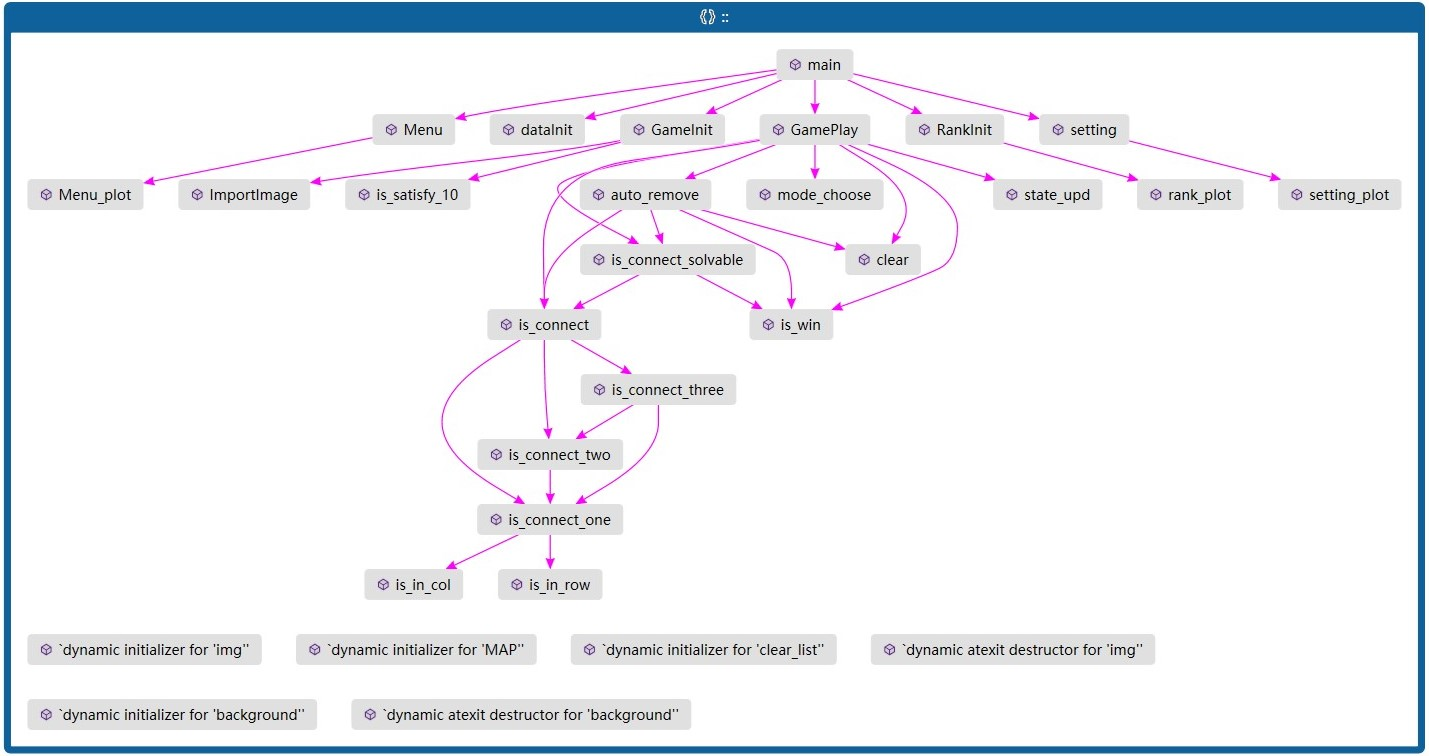
\includegraphics[width=1\textwidth]{code.jpg}
        \caption{函数调用关系} \label{fig:code}
    \end{figure}





